\chapter{Benchmark Specification}
\label{section:benchmark-specification}

\section{Requirements}

[TODO. This section will be filled after benchmark software is designed and
developed.]

%%%%%%%%%%%%%%%%%%%%%%%%%%%%%%%%%%%%%%%%%%%%%%%%%%%%%%%%%%%%%%%%%%%%%%%%%%%%%%
%%%%%%%%%%%%%%%%%%%%%%%%%%%%%%%%%%%%%%%%%%%%%%%%%%%%%%%%%%%%%%%%%%%%%%%%%%%%%%
%%%%%%%%%%%%%%%%%%%%%%%%%%%%%%%%%%%%%%%%%%%%%%%%%%%%%%%%%%%%%%%%%%%%%%%%%%%%%%

\section{Software and Useful Links}

[TODO. This section will be filled after benchmark software is designed and
developed.]

%%%%%%%%%%%%%%%%%%%%%%%%%%%%%%%%%%%%%%%%%%%%%%%%%%%%%%%%%%%%%%%%%%%%%%%%%%%%%%
%%%%%%%%%%%%%%%%%%%%%%%%%%%%%%%%%%%%%%%%%%%%%%%%%%%%%%%%%%%%%%%%%%%%%%%%%%%%%%
%%%%%%%%%%%%%%%%%%%%%%%%%%%%%%%%%%%%%%%%%%%%%%%%%%%%%%%%%%%%%%%%%%%%%%%%%%%%%%

\section{Data}

\subsection{Data Types}

\autoref{table:types} describes the different data types used in the benchmark.

\begin{table}[h]
\centering
\begin{tabular}{|>{\typeCell}p{\attributeColumnWidth}|p{\largeDescriptionColumnWidth}|}
    \hline
    \tableHeaderFirst{Type} & \tableHeader{Description} \\
    \hline
    ID & integer type with 64-bit precision. All IDs within a single entity type
    (e.g. Person) are unique, but different entity types (e.g. a Person and an
    Account) might have the same ID.\\
    \hline
    32-bit Integer &  integer type with 32-bit precision\\
    \hline
    64-bit Integer &  integer type with 64-bit precision\\
    \hline
    String & variable length text of size 40 Unicode characters\\
    \hline
    Long String & variable length text of size 256 Unicode characters\\
    \hline
    Text &  variable length text of size 2000 Unicode characters\\
    \hline
    Date &  date with a precision of a day, encoded as a string with the
    following format: \textit{yyyy-mm-dd}, where \textit{yyyy} is a four-digit
    integer representing the year, the year, \textit{mm} is a two-digit integer
    representing the month and \textit{dd} is a two-digit integer representing
    the day. \\
    \hline
    DateTime &  date with a precision of milliseconds, encoded as a string with
    the following format: \textit{yyyy-mm-ddTHH:MM:ss.sss+0000}, where
    \textit{yyyy} is a four-digit integer representing the year, the year,
    \textit{mm} is a two-digit integer representing the month and \textit{dd} is
    a two-digit integer representing the day, \textit{HH} is a two-digit integer
    representing the hour, \textit{MM} is a two digit integer representing the
    minute and \textit{ss.sss} is a five digit fixed point real number
    representing the seconds up to millisecond precision. Finally, the
    \textit{+0000} of the end represents the timezone, which in this case is
    always GMT.\\
    \hline
    Boolean &  logical type, taking the value of either True of False\\
    \hline
\end{tabular}
\caption{Description of the data types.}
\label{table:types}
\end{table}

\subsection{Data Schema}

\autoref{figure:schema} shows the data schema in UML. The schema defines the
structure of the data used in the benchmark in terms of entities and their
relations. Data represents a snapshot of the activity in several financial
scenarios during a period of time. The schema specifies different entities,
their attributes, and their relations. All of them are described in the
following sections.

\begin{figure}[htbp]
	\centering
	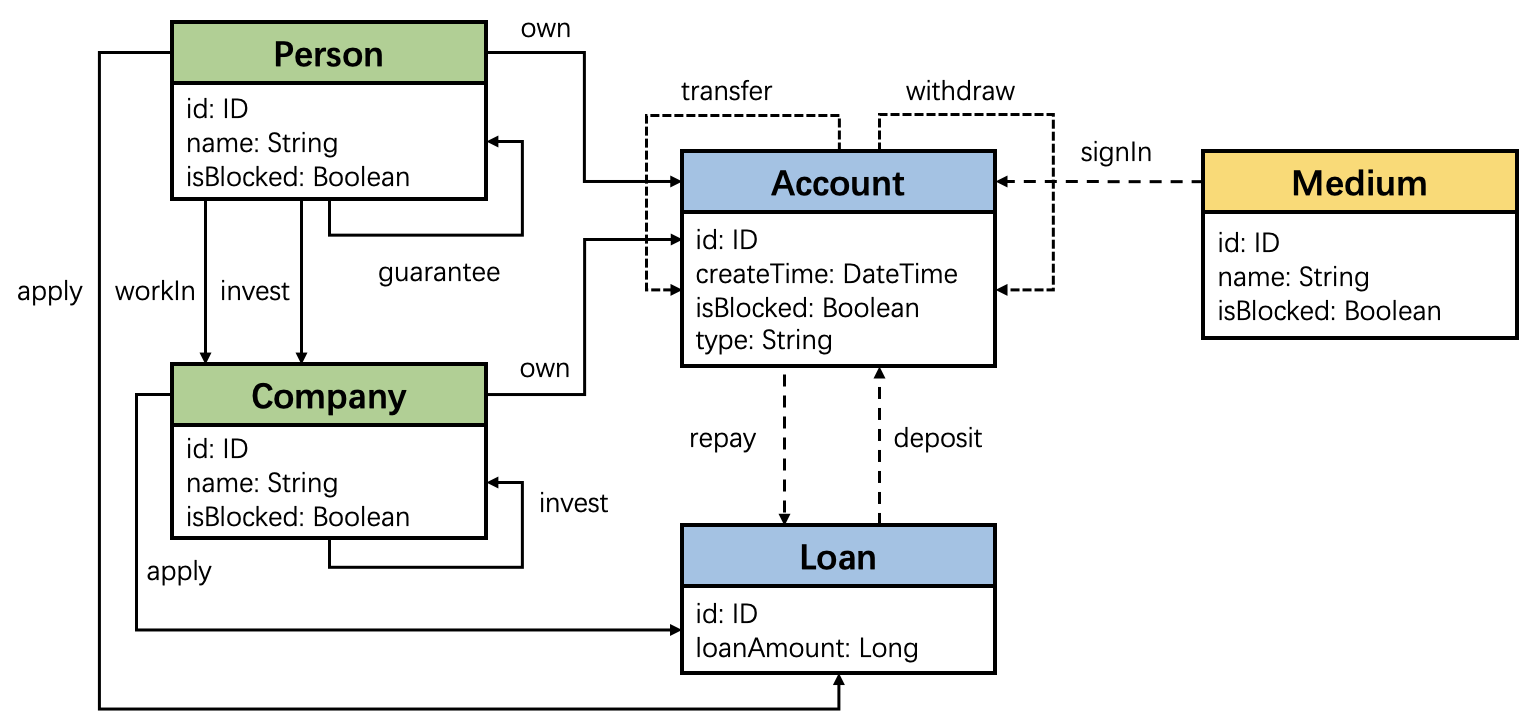
\includegraphics[width=\linewidth]{figures/data-schema}
	\caption{The \ldbcfinbench data schema}
	\label{figure:schema}
\end{figure}

Note: The dashed arrows in the schema represent multiple edges which means there
are more than one edge from start node to end node.

\subsubsection{Entities}

{\flushleft \textbf{Person:}} a person of the real world. \autoref{table:person}
shows the attributes.
\begin{table}[H]
    \begin{tabular}{|>{\varNameCell}p{\attributeColumnWidth}|>{\typeCell}p{\typeColumnWidth}|p{\descriptionColumnWidth}|}
        \hline
        \tableHeaderFirst{Attribute} & \tableHeader{Type} &
        \tableHeader{Description} \\
        \hline
        id & ID  & The identifier of the person.\\
        \hline
        name & String  & The name of the person.\\
        \hline
        isBlocked & Boolean  & If the person is blocked or concerned in
        systems.\\
        \hline
    \end{tabular}
    \caption{Attributes of Person entity.}
    \label{table:person}
\end{table}

{\flushleft \textbf{Company:}} a company of the real world, which persons work
in and persons invest. \autoref{table:company} shows the attributes.
\begin{table}[H]
    \begin{tabular}{|>{\varNameCell}p{\attributeColumnWidth}|>{\typeCell}p{\typeColumnWidth}|p{\descriptionColumnWidth}|}
        \hline
        \tableHeaderFirst{Attribute} & \tableHeader{Type} &
        \tableHeader{Description} \\
        \hline
        id & ID  & The identifier of the company.\\
        \hline
        name & String  & The name of the company.\\
        \hline
        isBlocked & Boolean  & If the company is blocked or concerned in
        systems.\\
        \hline
    \end{tabular}
    \caption{Attributes of Company entity.}
    \label{table:company}
\end{table}

{\flushleft \textbf{Account:}} an account in real world financial systems, which
is registered and owned by persons and companies. It includes many types such as
personalDeposit, personalCredit, etc. It can deal with other accounts.
\autoref{table:account} shows the attributes.
\begin{table}[H]
    \begin{tabular}{|>{\varNameCell}p{\attributeColumnWidth}|>{\typeCell}p{\typeColumnWidth}|p{\descriptionColumnWidth}|}
        \hline
        \tableHeaderFirst{Attribute} & \tableHeader{Type} &
        \tableHeader{Description} \\
        \hline
        id & ID  & The identifier of the account.\\
        \hline
        createTime & DateTime  & The time when the account created.\\
        \hline
        isBlocked & Boolean  & If the account is blocked or concerned in
        systems.\\
        \hline
        Type & String & The type of Account including personalDeposit,
        personalCredit, companyDeposit, card.\\
        \hline
    \end{tabular}
    \caption{Attributes of Company entity.}
    \label{table:account}
\end{table}

{\flushleft \textbf{Loan:}} a loan for persons and company to apply in real
world. \autoref{table:loan} shows the attributes.
\begin{table}[H]
    \begin{tabular}{|>{\varNameCell}p{\attributeColumnWidth}|>{\typeCell}p{\typeColumnWidth}|p{\descriptionColumnWidth}|}
        \hline
        \tableHeaderFirst{Attribute} & \tableHeader{Type} &
        \tableHeader{Description} \\
        \hline
        id & ID  & The identifier of the loan.\\
        \hline
        loanAmount & 64-bit Integer  & the amount of a loan\\
        \hline
    \end{tabular}
    \caption{Attributes of Company entity.}
    \label{table:loan}
\end{table}

{\flushleft \textbf{Medium:}} an abstract standing for things that users use to
sign in account in real world, such as IP, mac, phone numbers.
\autoref{table:medium} shows the attributes.
\begin{table}[H]
    \begin{tabular}{|>{\varNameCell}p{\attributeColumnWidth}|>{\typeCell}p{\typeColumnWidth}|p{\descriptionColumnWidth}|}
        \hline
        \tableHeaderFirst{Attribute} & \tableHeader{Type} &
        \tableHeader{Description} \\
        \hline
        id & ID  & The identifier of the medium.\\
        \hline
        name & String  & The name of the medium.\\
        \hline
        isBlocked & Boolean  & If the medium is blocked or concerned in
        systems.\\
        \hline
    \end{tabular}
    \caption{Attributes of Medium entity.}
    \label{table:medium}
\end{table}

\subsubsection{Relations}
Relations connect entities of different types.

\begin{longtable}{|>{\varNameCell}p{1.5cm}|>{\typeCell}p{2.5cm}|>{\typeCell}p{2.5cm}|>{\edgeDirectionCell}p{0.5cm}|p{6cm}|}
        \hline
        \tableHeaderFirst{Name} & \tableHeader{Tail} & \tableHeader{Head} & \tableHeader{Multiplicity} & \tableHeader{Description} \\
        \hline
        signIn & Medium & Account & N & An account is signed in with a Media 1.timestamp: DateTime \\
        \hline
        own & Person/Company & Account & 1 & A person or a company owns an account. \\
        \hline
        transfer & Account & Account & N & Fund transfers between two accounts. 1.timestamp: DateTime 2.amount: 64-bit Integer\\
        \hline
        deposit & Loan & Account & N & Loan fund is deposited to an account	1. timestamp: DateTime 2. amount: 64-bit Integer \\
        \hline
        repay & Account & Loan & N & Loan is repaid from an account	1. timestamp: DateTime 2. amount: 64-bit Integer \\
        \hline
        withdraw & Account & Account & N & Fund is transferred from an account to another account whose type is card	1. timestamp: DateTime 2. amount: 64-bit Integer \\
        \hline
        invest & Person/Company & Company & 1 & A person or a company invests a company	1. timestamp: DateTime 2. percent: Float \\
        \hline
        workIn & Person & Company & 1 & A person works in a company	/ \\
        \hline
        apply & Person/Company & Loan & 1 & A person or a company applies a Loan. 1. timestamp: DateTime \\
        \hline
        guarantee & Person & Person & 1 & A person guarantees another for some reason like loans. 1. timestamp: DateTime \\
        \hline
        \caption{Description of the data relations.}
        \label{table:relations}
\end{longtable}

\subsection{Data Generation}
[TODO. This section will be filled after benchmark software designed and developed.]

\subsection{Output Data}
[TODO. This section will be filled after benchmark software designed and developed.]\

%%%%%%%%%%%%%%%%%%%%%%%%%%%%%%%%%%%%%%%%%%%%%%%%%%%%%%%%%%%%%%%%%%%%%%%%%%%%%%
%%%%%%%%%%%%%%%%%%%%%%%%%%%%%%%%%%%%%%%%%%%%%%%%%%%%%%%%%%%%%%%%%%%%%%%%%%%%%%
%%%%%%%%%%%%%%%%%%%%%%%%%%%%%%%%%%%%%%%%%%%%%%%%%%%%%%%%%%%%%%%%%%%%%%%%%%%%%%

\section{Benchmark Workflow}
[TODO. This section will be filled after benchmark software designed and developed.]

%%%%%%%%%%%%%%%%%%%%%%%%%%%%%%%%%%%%%%%%%%%%%%%%%%%%%%%%%%%%%%%%%%%%%%%%%%%%%%
%%%%%%%%%%%%%%%%%%%%%%%%%%%%%%%%%%%%%%%%%%%%%%%%%%%%%%%%%%%%%%%%%%%%%%%%%%%%%%
%%%%%%%%%%%%%%%%%%%%%%%%%%%%%%%%%%%%%%%%%%%%%%%%%%%%%%%%%%%%%%%%%%%%%%%%%%%%%%
